\documentclass{article}
\usepackage{multicol}
\usepackage{calc}
\usepackage{ifthen}
\usepackage[margin=0.5in]{geometry}
\usepackage{amsmath,amsthm,amsfonts,amssymb}
\usepackage{esint}
\usepackage{amsfonts}
\usepackage{color,overpic}
\usepackage{hyperref}
\usepackage{array} 
\usepackage{amstext}
\usepackage{enumitem}
\usepackage{graphicx}
\usepackage{caption}
\usepackage{natbib}

\newenvironment{Figure}
  {\par\medskip\noindent\minipage{\linewidth}}
  {\endminipage\par\medskip}
  
  
% Turn off header and footer
%\pagestyle{empty}



% -----------------------------------------------------------------------

\begin{document}
\begin{multicols}{2}

\setlist[itemize]{leftmargin=*} % set itemise indentation to leftmargin
\setlist[enumerate]{leftmargin=*}


\begin{center}
     \Large{\underline{Gradual Deformation Method }} \\
\end{center}

\section{Introduction}

Gradual Deformation Method (GDM) is an History Matching Method (HMM) (or Calibration) from the family of deformation Technique. 

\subsection{Objetif}
The general objective of HMM is the conditioning the model to data, which is formulate as an optimization problem. An objectif function is created to measure the misfit and  the target of the method is to minimized it. 
A Good technique should :
\begin{itemize}
\item Respect spacial continuity and structure (2-pts or multipoint)
\item Have me most regular OF (use of Gradient Based  (GB) technique improve computation effort)
\item Cover the whole solution space
\end{itemize}


\subsection{Other technique}
\begin{itemize}
\item “Swaping Value”, “Genetic Operation” \citep{deutsch1993conditioning} But they violate spacial continuity.
\item  simulated annealing or genetic algorithms 
\item “Conditional simulation” \citep{Oliver1997} : Very slow OF convergence
\item “Pilot Point Method” \citep{de1984interpretation} (use of conditioning kriging \citep{journel1978mining}): + : minimial nb of parm., use of GB opt. Algo. - : degradation of spacial structure when pilote point too close.
\item “Visualizing Uncertainty” \citep{srivastava1994interactive} (generate lager grid solution and moving the grid in the model) pb when large model
\end{itemize}

\subsection{History and Developement}
\begin{enumerate}
\item \cite{Hu2000} explain in detail GDM.
\item \cite{Hu2001} show application for iterative calibration of Sequential (not necessarly Gaussian) Simulation
\item \cite{LeRavalec-Dupin2002} look at gradient based gradual deformation with uncertainty.
\item \cite{Hu2002} generalized GDM to dependant relalizations. He looked at conditioning before deforme and combine correlated field.
\item \cite{Hu2004} explore a gradient based compounding procedure to explore faster the space
\end{enumerate}
Other paper include : \cite{hu1998constraining, roggero1998gradual, LeRavalec2000} and Ravalec-Dupin Book's.



\section{Basic Description}
\subsection{Gaussian related Stochastic models}
$Z(\mathbf{x})$ is the physical property of interest at location $\mathbf{x}$. Let $Y(\mathbf{x})$ be a stationary standard Gaussian ($ \mathcal{N}(0,1)$) random function. $G$ and $F$ are the distribution function of $Y$ and $Z$ respectively. 
\[ Z(\mathbf{x}) = F^{-1}{G[Y(\mathbf{x})]} \]
The idea behind the equation is the build the field from a standard normally distributed field. For exemple, if $Z$ is the hydraulic conductivity (K), $F(Z)$ would be the $\log(K)$, and $G(Y)$ would simply be: $m + \sigma Y$. Such that : \[ Z(\mathbf{x}) = \exp(m + \sigma Y) \]

\subsection{Gradual Deformation}
The idea is to deform a field $Y_1$ into $Y(\theta)$ using another field $Y_2$ and a parameter $\theta$. What is magical is that $Y$ will preserve the std normal distribution of $Y1$. It's important to note that $Y_1$ and $Y_2$ are  std normally distributed ($ \mathcal{N}(0,1)$) (also called standard gaussian or white noise)
\[Y( \theta) = Y_1 \cos ( \theta) + Y_2 \sin ( \theta)\]
\begin{Figure}
 \centering
 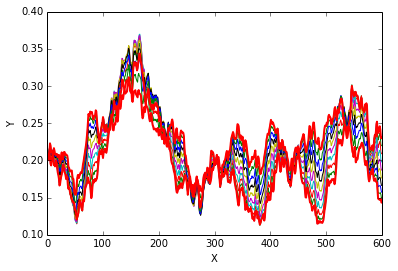
\includegraphics[width=\linewidth]{grad-1.png}
 \captionof{figure}{Exemple of 1D Gradual deformation. Thick red line are $Y_1$ and $Y_2$. Other line are deformation with various $\theta$ value}
\end{Figure}

An graphical interpretation of gradual deformation is to view the equation as an ellipse equation, when Y dimension is two.
\begin{Figure}
 \centering
 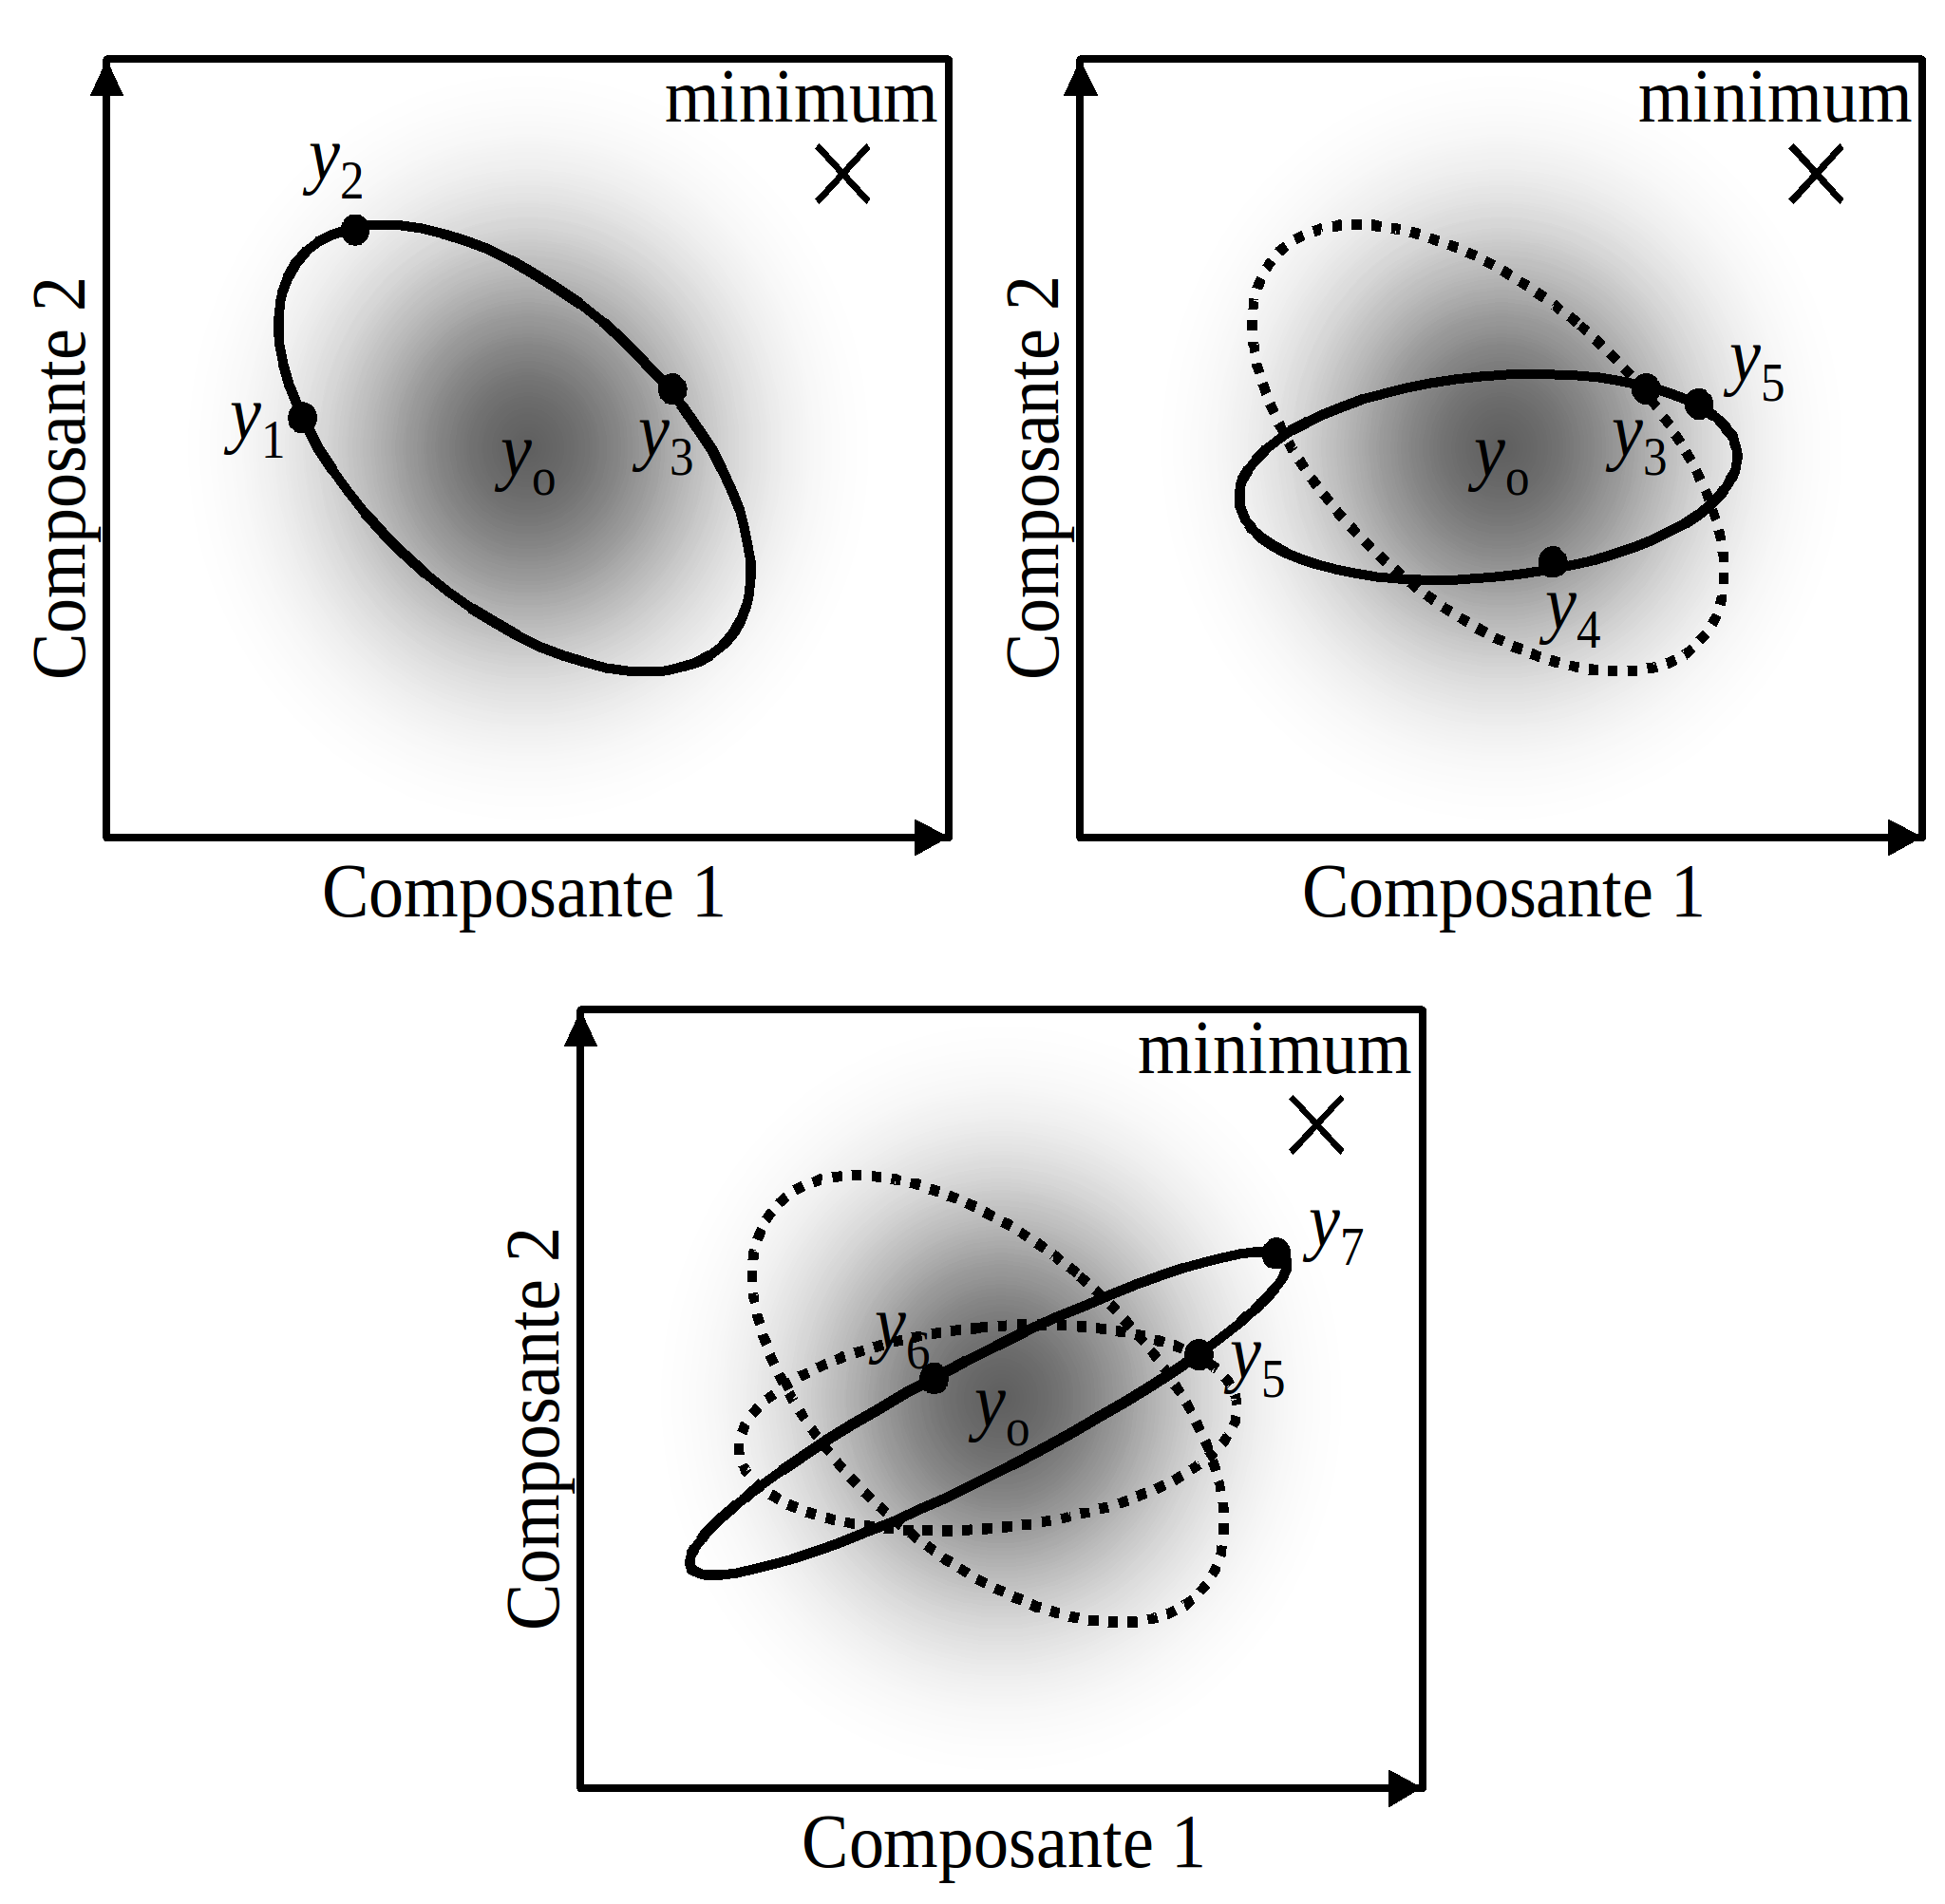
\includegraphics[width=\linewidth]{grad_def_ex_8.png}
 \captionof{figure}{Graphical illustration of Gradual Deformation}
\end{Figure}



\section{Extension}
\subsection{Structural parameter}
Often the hard data are not enough to give the structure (variance, covariance, mean...) and \textit{a priori} distribution need to be assumed. The Trick here is to transform the field $Y(\theta)$ into  a new field $X(\theta)=L[Y(\theta)]$ which impose the structure (covariance). Algo such as Cholesky (LU decomposition), FFT-MA or moving average can do that

\subsection{Conditioning Kriging}
Incorporation of "hard data" can done using conditional kriging. The integration of this data is on the field $Y$ not $Y_1$ or $Y_2$
\[Y_c (\mathbf{x}) = Y_{dk} (\mathbf{x}) + [Y(\mathbf{x}) − Y_k (\mathbf{x})] \]
Where $Y_c$ is the resulting simulation, $Y_{dk}$ is the kriged data, $Y$ the unconditionned simulation and $Y_k$ the krigeage of the result of uncondition simulation ($Z$) at the known data point.
Ying and Gomez-Hernandez, 2000 propose to combine directly conditional realization before deformation. (reframe in \cite{Hu2002})


\subsection{Multidimentional Gradual Deformation}
see \cite{Hu2000} or \cite{LeRavalec-Dupin2002}. GDM can be extend to more than two gradual deformation.
\[ Y(\theta_i , i \in [1,S] ) = \prod_{i=1}^S Y_1 \cos (\theta_i)    + \sum_{i=1}^S \sin (\theta_i) \prod_{j=i+1}^S Y_i+1 \cos (\theta_j) \]

\subsection{Indicator variable}
can be used for binary variable...

\subsection{Local and Regionalized}
see \cite{Hu2000}.
\begin{Figure}
 \centering
 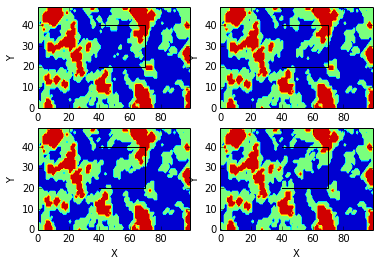
\includegraphics[width=\linewidth]{grad_def_ex_2}
 \captionof{figure}{Exemple of 2D Local Gradual deformation.}
\end{Figure}

\subsection{Way to combine them}
see \cite{Hu2004}.
GDM is often loop to improve at each iteration the solution. Three way of combining exist:
\[ Y_{n+1}(\theta)  = Y_{n}(\theta) \cos (\theta)  + U_{new} \sin (\theta)\]
\begin{enumerate}
\item $Y_{n+1} = GDM(Y_{n}, U)$ : (fig A)
\item $Y_{n+1} = GDM(Y_{n}, U_{1, 2...})$ : (fig B) use the Multidimentional GDM
\item $Y_{n+1} = GDM(Y_{n}, GBC(U_{1, 2...}))$ : (fig C). Use a linear combination of $U_i$ (Gradient Based Compounding) such that the gradient search is the closest to the gradient search direction. This require the OF to be differentiable.
\end{enumerate}
See graph to understand. The method on the right converge very quickly to a local optima without finding the whole space. The second method was then proposed, it uses multidimensional gradual deformation. It is also slow.

\begin{Figure}
 \centering
 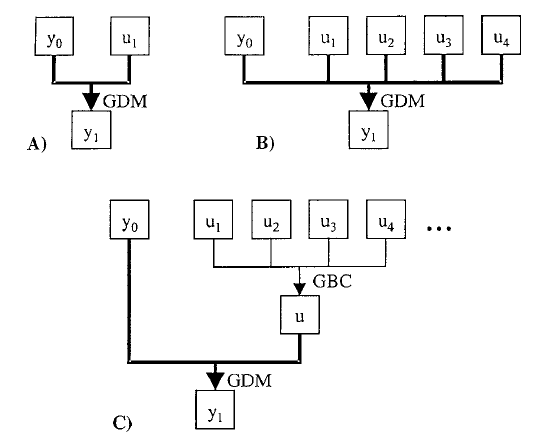
\includegraphics[width=\linewidth]{grad_def_ex_12}
 \captionof{figure}{Three way to combine realizations}
\end{Figure}




\section{General Utilisation}
\subsection{History Matching}
As usual, minimize an objectif function (OF) 
\[ J(\theta) = \frac{1}{p} \sum_{i=1}^{p} \omega_i (f_i(Z(Y(\theta))) - f_i^{obs})^2 \]
 where an function $f$ depend on the field $Z$ and therefore on the gaussian field deformated $Y(\theta)$. The optimization procedure is to find $\theta_{opt}$ which minimize $O$.

Efficient optimization procedure require the OF to be derivable in regard to $\theta$ (Gradient Based Method). Otherwise, other method such as Golden Search (require monotonic function). \cite{Hu2000} suggest not to limit $\theta$ to $[0,\pi/2]$ (his period) as optimization search often exclude search at their limit (Golden search by instance).

\subsection{Advance Optimization: Prior constraint}
(see \citep{LeRavalec-Dupin2002})
This optimization problem is often ill posed (not one unique solution, measurement error, model error...). Extra information can be add to the OF to help convergence (Regularization, Neuman, 1973). The model ($p$) can have prior estimate $p_0$ to be constraint to. $\alpha$ is giving the relative importance of this prior estimate
\[ J(p)  = \sum_i \omega_i (f_i-f_i^{obs})^2   + \alpha \sum_i v_i (p_i-p_{0,i})^2\]

\subsection{Iterative Calibration of Sequential (not necessary Gaussian) Simulation}
see \cite{Hu2001}.
In sequential simulation, the order to visit each cell is randomly generated ($U$). At each location $i$, $z(u_i)$ is sampled from a distribution conditioned by the previously simulated point and hard data ($pdf(Z_i =z_i)$). In order make the sampling easier, cumulative distributed function (cdf) is build. $z_i$ is obtain with $z_i=CDF^{-1}(v_i)$ where $v_i$ is sampled in a uniform distribution [0,1]. From this point of view, sequential simulation can be view as transforming a uniform sampled points $V$ into a field $Z$. As GDM require a std normally dist. field ($Y$) to be deform, $V$ need to be generated from $Y$. This is easily done using the normal cumulative distribution function (normcdf). We end up with a similar optimization problem (calibration) as before : field $Y$ to deform to get better OF.

\subsection{Uncertainty}
see \cite{LeRavalec-Dupin2002,LeRavalec2000}

\subsection{Combining Dependant Realization}
see \cite{Hu2002}.
$Y_i$ are still (multi-) gaussian random function. They have a covariance function $C(h)$ and their cross-covariance function is proportional to $C(h)$
\[ C_{ij}(h) = E[Y_i(x) Y_j(x+h)] = r_{ij} C(h)\]
where $r_{ij}$ stand for the correlation coef. between $Y_i$ and $Y_j$. The covariance of a linear combinaison $Y(x) = \sum_i \alpha_i Y_i$ will therefore be :
\[ 
\begin{array}{ll}
 C_Y (h) &= E[Y(x) Y(x+h)] \\
         &= E \left[ \left( \sum_i \alpha_i Y_i(x) \right) \left( \sum_j \alpha_j Y_j(x+h) \right) \right] \\
         &= E\left[\left(\sum_i \sum_j \alpha_i \alpha_j Y_i(x) Y_j(x+h)    \right)\right] \\
         &= C(h) \sum_{i,j} r_{ij} \alpha_i \alpha_j 
\end{array}
\]
To maintain the same covariance, we need $\sum_{i,j} r_{ij} \alpha_i \alpha_j =1$. This can be shown to be a generalisation of GDM for dependant realization. 
One idea in his paper was to transform each realization to force a mean of zero and standard deviation of 1 : $Y_i^*=\frac{Y_i-\bar{Y_i}}{\sigma_{Y_i}}$


\section{Limitation}
\begin{itemize}
\item 1st order stationary (mean cst) required
\item Only applicable for Gaussian-related stochastic model
\item if search long enough : global minima is achieved.
\item In theory, spacial structure is preserve. But in practise, because each simulation is not perfect (exact mean, variance and covariance) spatial statistical structure is not preserve. This become a serious problem when the number of realisation is higher than the number of grid cells (see \cite{Hu2002})
\item Preserve only variogram structure (covariance) not multi-point
\item for linear problems, GDM's optimizations  converge exponentially to the global minimum but not for non linear. 
\item Something about getting accurate estimate... using a prior constraint \cite{LeRavalec-Dupin2002}
\end{itemize}

\section{To go futher}
\begin{itemize}
\item Grdual Pilote Point (book)
\item Probability Perturbation Method
\end{itemize}




\bibliographystyle{apalike}
\bibliography{citations}	
	
\end{multicols}

\end{document}
